\documentclass[10pt]{beamer}

\usepackage[]{graphicx}
\usepackage[]{color}

\usepackage{alltt}

% Beamer themer
%\usetheme{metropolis}
\usetheme{Warsaw}
\setbeamertemplate{navigation symbols}{}
% \setbeamertemplate{footline}[frame number]
\expandafter\def\expandafter\insertshorttitle\expandafter{%
  \insertshorttitle\hfill%
  \insertframenumber\,/\,\inserttotalframenumber}

\usepackage{graphicx}

\usepackage{listings}
\lstset
{
    % language=[LaTeX]TeX,
    breaklines=true,
    basicstyle=\tt\scriptsize,
    keywordstyle=\color{blue},
    identifierstyle=\color{magenta},
}

\DeclareGraphicsExtensions{.pdf,.jpeg,.jpg,.png}

\usepackage{subcaption}
\usepackage{amsmath}

\usepackage[authoryear]{natbib}

\usepackage{tikz}
\usetikzlibrary{calc}
% \usetikzlibrary{bayesnet}
% \usepackage{pgfplots}
% \pgfplotsset{compat=1.13}
\usetikzlibrary{math}

\usepackage[framemethod=TikZ, xcolor=RGB]{mdframed}
\definecolor{mydarkblue}{rgb}{0,.06,.5}
\definecolor{mydarkred}{rgb}{.5,0,.1}
\definecolor{myroyalblue}{rgb}{0,.1,.8}
\mdfdefinestyle{MyFrame}{%
    linecolor=mydarkblue,
    outerlinewidth=0.5pt,
    roundcorner=2pt,
    innertopmargin=2pt,
    innerbottommargin=2pt,
    innerrightmargin=2pt,
    innerleftmargin=2pt,
    backgroundcolor=blue!10}

% Set a transparent background to match ggplot figures
\setbeamercolor{background canvas}{bg=}

\usepackage{xargs} % For def with default arguments
\usepackage{mathrsfs} % For mathscr

\usepackage{amssymb}
\usepackage{amsmath}
\usepackage{amsthm}
\usepackage{mathtools}

% https://tex.stackexchange.com/questions/89166/centering-in-tabularx-and-x-columns
\usepackage{tabularx}   % For horizontally filled tables
\newcolumntype{Y}{>{\centering\arraybackslash}X}
\usepackage{booktabs}    % For toprule among other things

\usepackage{refstyle}
\usepackage{varioref} % Use refstyle instead of varioref directly.

% Math definitions

% Some definitions for the text

\def\loset{MIS}
\def\loeff{MIP}
\def\loalpha{PIP}
\def\aloset{AMIS}
\def\aloeff{AMIP}
\def\aloalpha{APIP}
\def\na{\texttt{NA}}

%%%%%%%%%%%%%%%%%%%%%%%%
% Rachael's math defs

\DeclareMathOperator*{\argmax}{arg\,max}
\DeclareMathOperator*{\argmin}{arg\,min}

\DeclarePairedDelimiter\abs{\lvert}{\rvert}
\DeclarePairedDelimiter\norm{\lVert}{\rVert}

% Swap the definition of \abs* and \norm*, so that \abs
% and \norm resizes the size of the brackets, and the
% starred version does not.
\makeatletter
\let\oldabs\abs
\def\abs{\@ifstar{\oldabs}{\oldabs*}}

%\let\oldnorm\norm
\def\norm{\@ifstar{\oldnorm}{\oldnorm*}}

%%%%%%%%%%%%%%%%%%%%%%%%
% Ryan's math defs


% \norm was taken, so use \vnorm for "vector norm".
\global\long\def\info{\mathcal{I}}%

% These are all used for the finite sample bounds section.
\global\long\def\betalin{\hat\beta^{\mathrm{lin}}}%
\global\long\def\nset{\mathcal{S}}%

\global\long\def\cop{C_{op}}%
\global\long\def\cmoment{H_2}%
\global\long\def\cxxlo{\xi_1}%
\global\long\def\cxepslo{\xi_2}%
\global\long\def\cball{\mathscr{B}}%
\global\long\def\cijdiff{\Delta_{lin}}%

\global\long\def\copscaled{\tilde{C}_{op}}%

% calculus
\newcommand{\dee}{\mathrm{d}}

% Influence score and related quantities
\def\infl{\psi}
\def\inflscale{\hat{\sigma}_{\infl}}
\def\inflscalelim{\sigma_{\infl}}
\def\ind#1{\mathbb{I}\left(#1\right)}
\def\mis#1{S_{#1}}
\def\mip#1{\Psi_{#1}}
\def\amis#1{\hat{S}_{#1}}
\def\amip#1{\hat{\Psi}_{#1}}
\def\loprop#1{\alpha^*_{#1}}
\def\aloprop#1{\hat{\alpha}^*_{#1}}
\def\thetafun{\phi}
\def\thetafunlin{\thetafun^{\mathrm{lin}}}%
\def\thetalin{\thetahat^{\mathrm{lin}}}%

\def\shape{\mathcal{S}_\alpha}
\def\noise{\hat\sigma_{\phi}}
\def\plim{\overset{p}{\rightarrow}}

% Vectors
%\def\x{\vec{x}}
\def\d{d} % A general data point
\def\p{p} % The index into the parameter vector
\def\P{P} % The length of the parameter vector
\def\w{\vec{w}}
\def\wnorm{\vec{\omega}} % Used only in the \thetafun lemma

\def\zP{0_{\P}}
\def\zPN{0_{\P \times N}}
\def\thetahat{\hat{\theta}}
\def\onevec{\vec{1}}
\def\inflvec{\vec{\infl}}

% Operators
\def\sumn{\sum_{n=1}^N}
\def\meann{\frac{1}{N}\sum_{n=1}^N}
\def\var#1{\mathrm{Var}\left(#1\right)}
\def\vnorm#1{\left\Vert #1\right\Vert }%
\def\falphanorm#1#2{\left\Vert #2\right\Vert_{#1, \alpha} }%
\def\at#1#2{\left.#1\right|_{#2}}%
\def\fracat#1#2#3{\at{\frac{#1}{#2}}{#3}}%
\def\mbe{\mathbb{E}}%
\def\argmaxover#1{\underset{#1}{\mathrm{argmax}}\,}
\def\maxover#1{\underset{#1}{\mathrm{max}}\,}

% This file contains the boilerplate that knitr would put at the top of
% a knitr document if you ran knitr with \begin{document} ... \end{document}.
% By including it once in the main document, you can knit and \input{}
% Rnw files that contain only individual sections.

\usepackage[]{graphicx}
\usepackage[]{color}
%% maxwidth is the original width if it is less than linewidth
%% otherwise use linewidth (to make sure the graphics do not exceed the margin)
\makeatletter
\def\maxwidth{ %
  \ifdim\Gin@nat@width>\linewidth
    \linewidth
  \else
    \Gin@nat@width
  \fi
}
\makeatother

\definecolor{fgcolor}{rgb}{0.345, 0.345, 0.345}
\newcommand{\hlnum}[1]{\textcolor[rgb]{0.686,0.059,0.569}{#1}}%
\newcommand{\hlstr}[1]{\textcolor[rgb]{0.192,0.494,0.8}{#1}}%
\newcommand{\hlcom}[1]{\textcolor[rgb]{0.678,0.584,0.686}{\textit{#1}}}%
\newcommand{\hlopt}[1]{\textcolor[rgb]{0,0,0}{#1}}%
\newcommand{\hlstd}[1]{\textcolor[rgb]{0.345,0.345,0.345}{#1}}%
\newcommand{\hlkwa}[1]{\textcolor[rgb]{0.161,0.373,0.58}{\textbf{#1}}}%
\newcommand{\hlkwb}[1]{\textcolor[rgb]{0.69,0.353,0.396}{#1}}%
\newcommand{\hlkwc}[1]{\textcolor[rgb]{0.333,0.667,0.333}{#1}}%
\newcommand{\hlkwd}[1]{\textcolor[rgb]{0.737,0.353,0.396}{\textbf{#1}}}%
\let\hlipl\hlkwb

\usepackage{framed}
\makeatletter
\newenvironment{kframe}{%
 \def\at@end@of@kframe{}%
 \ifinner\ifhmode%
  \def\at@end@of@kframe{\end{minipage}}%
  \begin{minipage}{\columnwidth}%
 \fi\fi%
 \def\FrameCommand##1{\hskip\@totalleftmargin \hskip-\fboxsep
 \colorbox{shadecolor}{##1}\hskip-\fboxsep
     % There is no \\@totalrightmargin, so:
     \hskip-\linewidth \hskip-\@totalleftmargin \hskip\columnwidth}%
 \MakeFramed {\advance\hsize-\width
   \@totalleftmargin\z@ \linewidth\hsize
   \@setminipage}}%
 {\par\unskip\endMakeFramed%
 \at@end@of@kframe}
\makeatother

\definecolor{shadecolor}{rgb}{.97, .97, .97}
\definecolor{messagecolor}{rgb}{0, 0, 0}
\definecolor{warningcolor}{rgb}{1, 0, 1}
\definecolor{errorcolor}{rgb}{1, 0, 0}
\newenvironment{knitrout}{}{} % an empty environment to be redefined in TeX

\usepackage{alltt}

%%%%%%%%%%%%%%%%%%%%%%%%%%%%%%%%%%%%%%
%%%%%%%%%%%%%%%%%%%%%%%%%%%%%%%%%%%%%%
% Do not edit the TeX file your work
% will be overwritten.  Edit the RnW
% file instead.
%%%%%%%%%%%%%%%%%%%%%%%%%%%%%%%%%%%%%%
%%%%%%%%%%%%%%%%%%%%%%%%%%%%%%%%%%%%%%





%%%%%%%%%%%%%%%%%%%%%%
%%%%%%%%%%%%%%%%%%%%%%
%%%%%%%%%%%%%%%%%%%%%%
% Plots

\newcommand{\BaseHistogram}{
\begin{knitrout}
\definecolor{shadecolor}{rgb}{0.969, 0.969, 0.969}\color{fgcolor}

{\centering 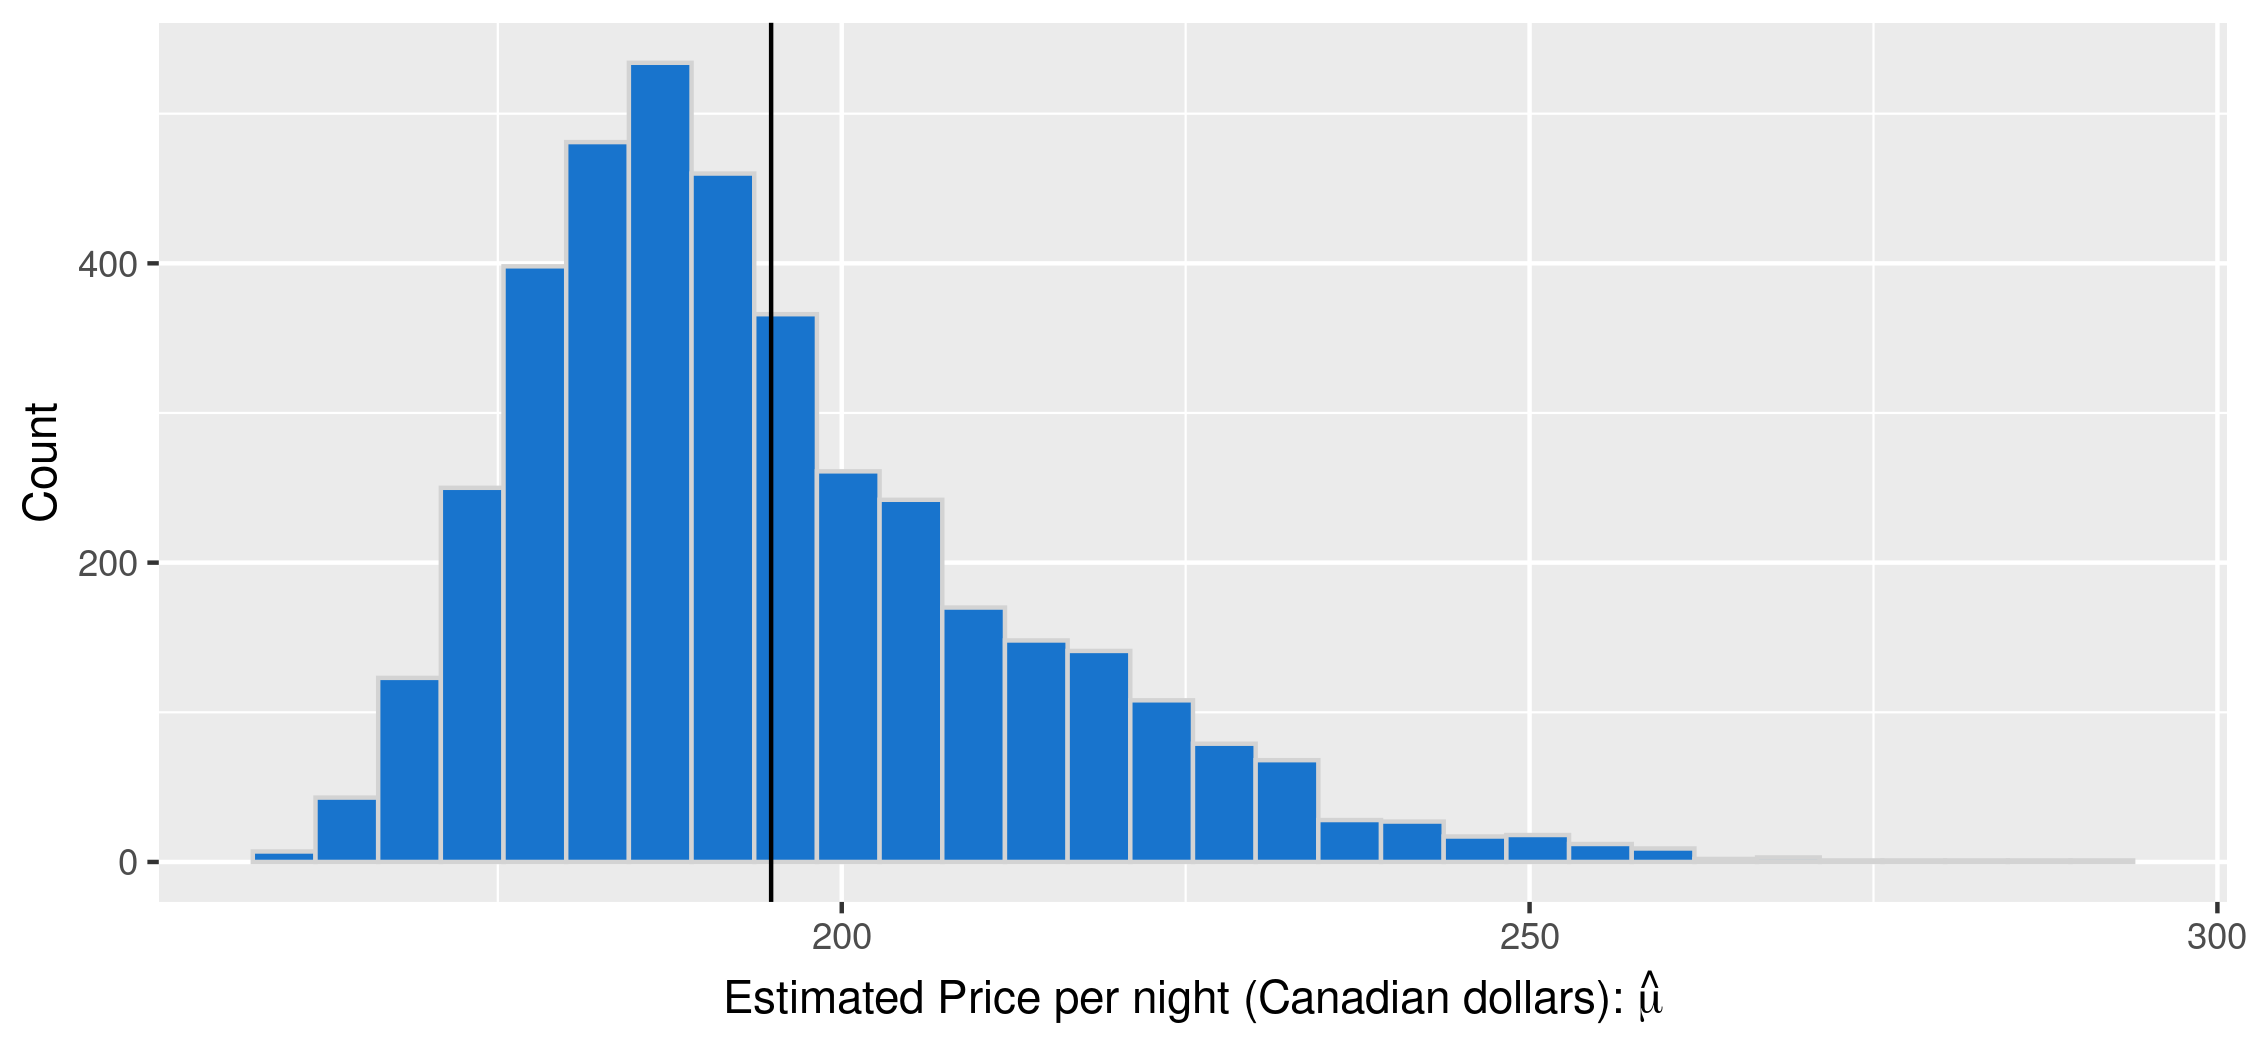
\includegraphics[width=0.98\linewidth,height=0.461\linewidth]{figure/base-hist-1} 

}



\end{knitrout}
}


\newcommand{\BaseHistogramWithArrow}{
\begin{knitrout}
\definecolor{shadecolor}{rgb}{0.969, 0.969, 0.969}\color{fgcolor}

{\centering 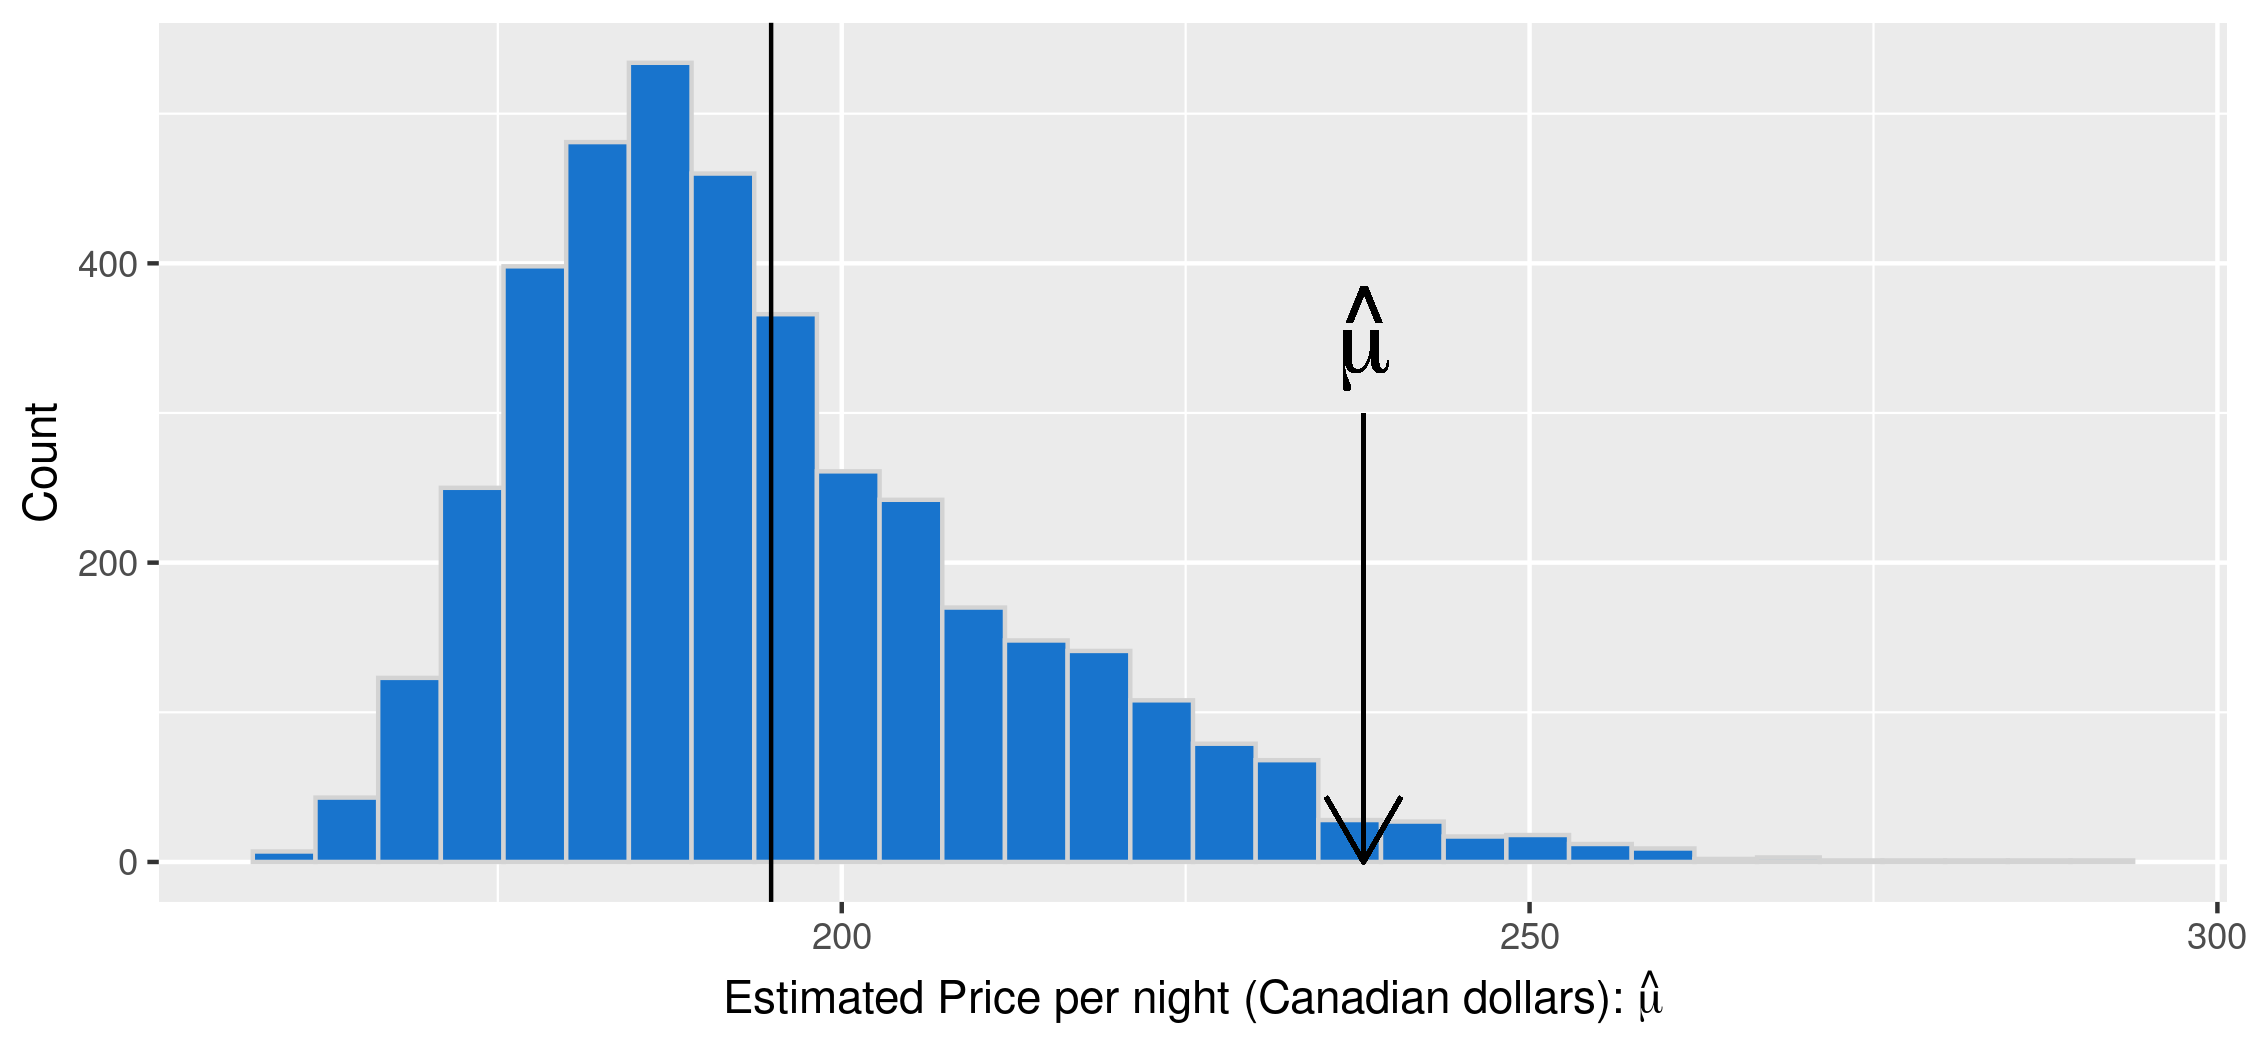
\includegraphics[width=0.98\linewidth,height=0.461\linewidth]{figure/base-hist-arrow-1} 

}



\end{knitrout}
}



\newcommand{\BaseHistogramFaded}{
\begin{knitrout}
\definecolor{shadecolor}{rgb}{0.969, 0.969, 0.969}\color{fgcolor}

{\centering 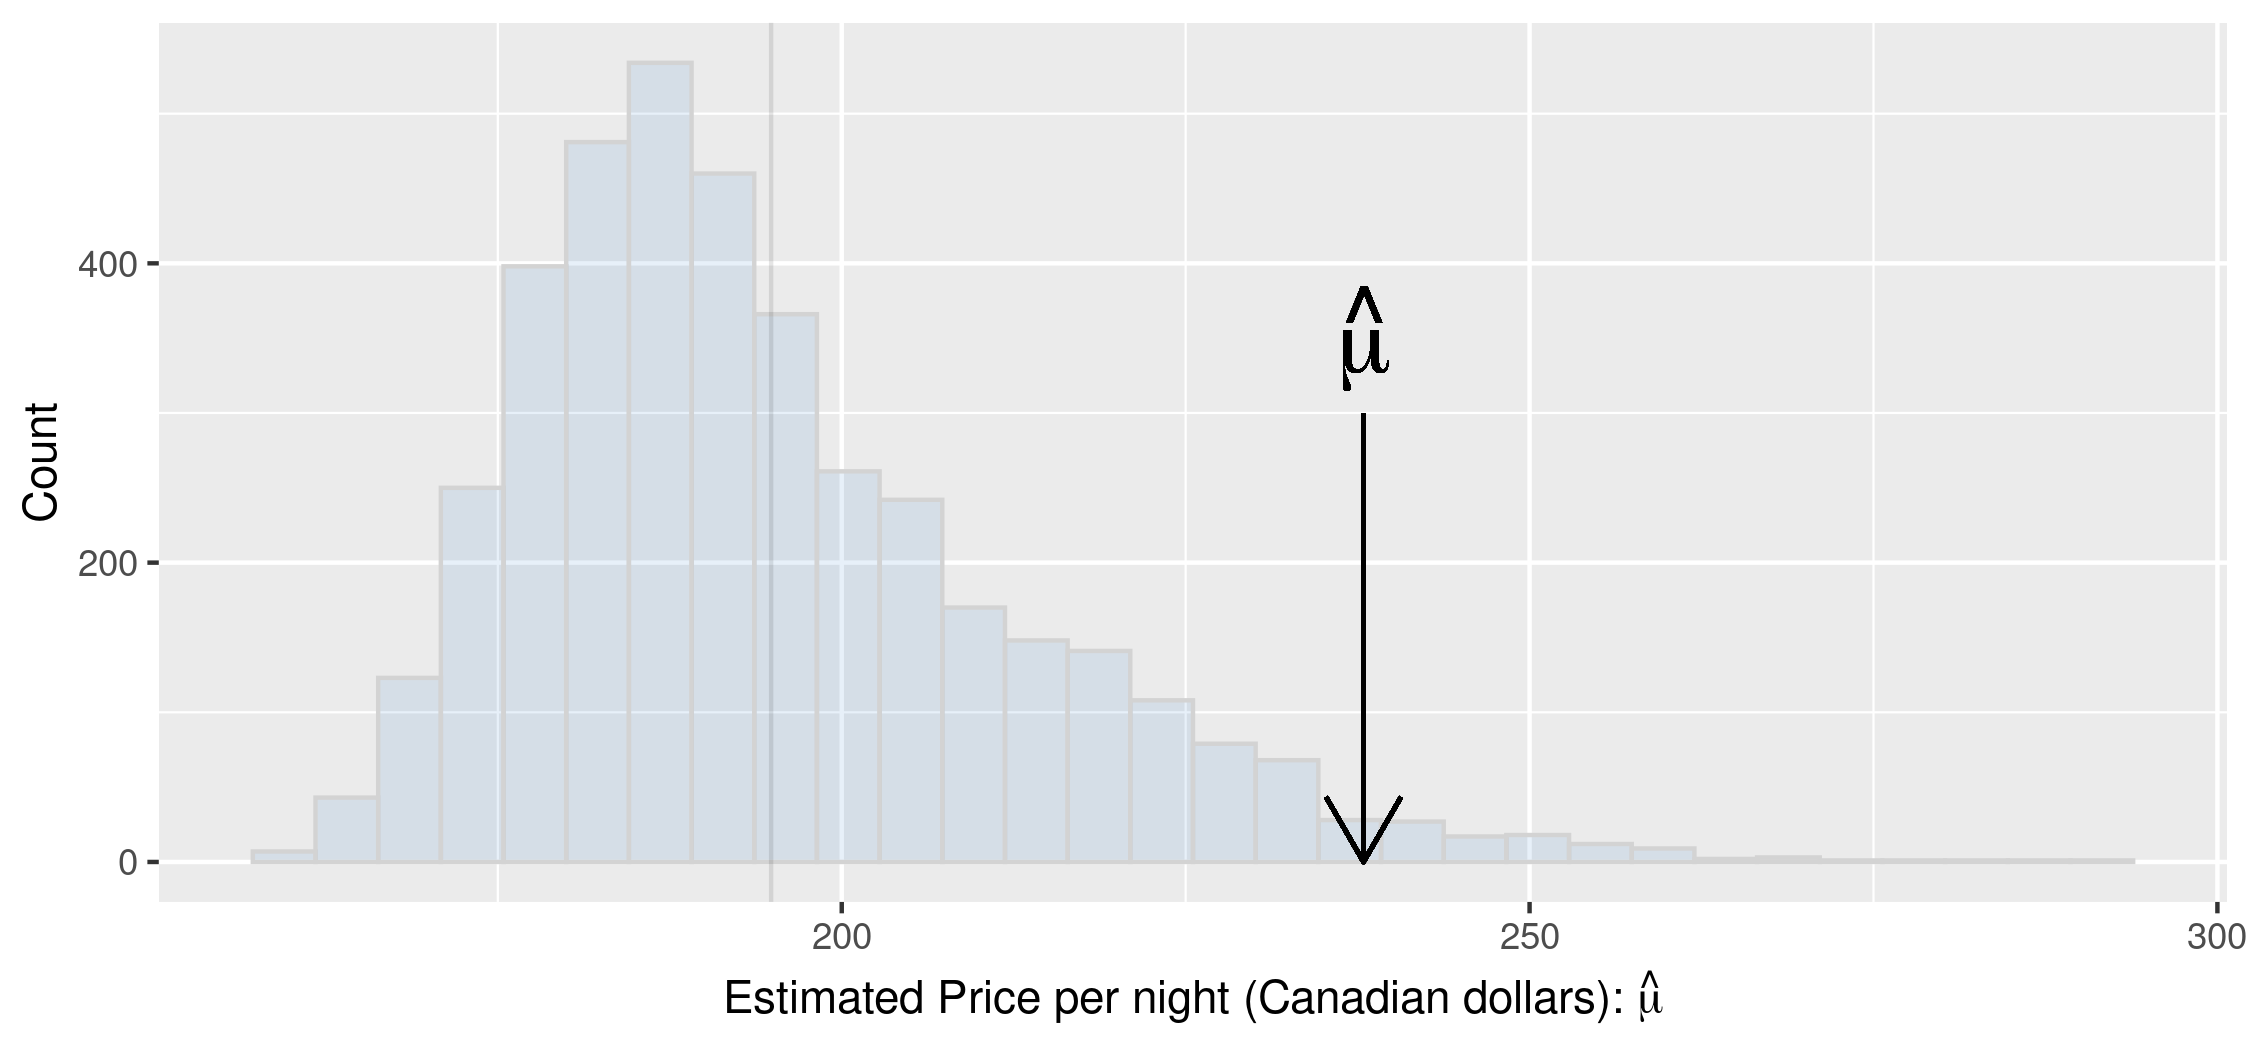
\includegraphics[width=0.98\linewidth,height=0.461\linewidth]{figure/base-hist-faded-1} 

}



\end{knitrout}
}


\newcommand{\SingleCI}{
\begin{knitrout}
\definecolor{shadecolor}{rgb}{0.969, 0.969, 0.969}\color{fgcolor}

{\centering 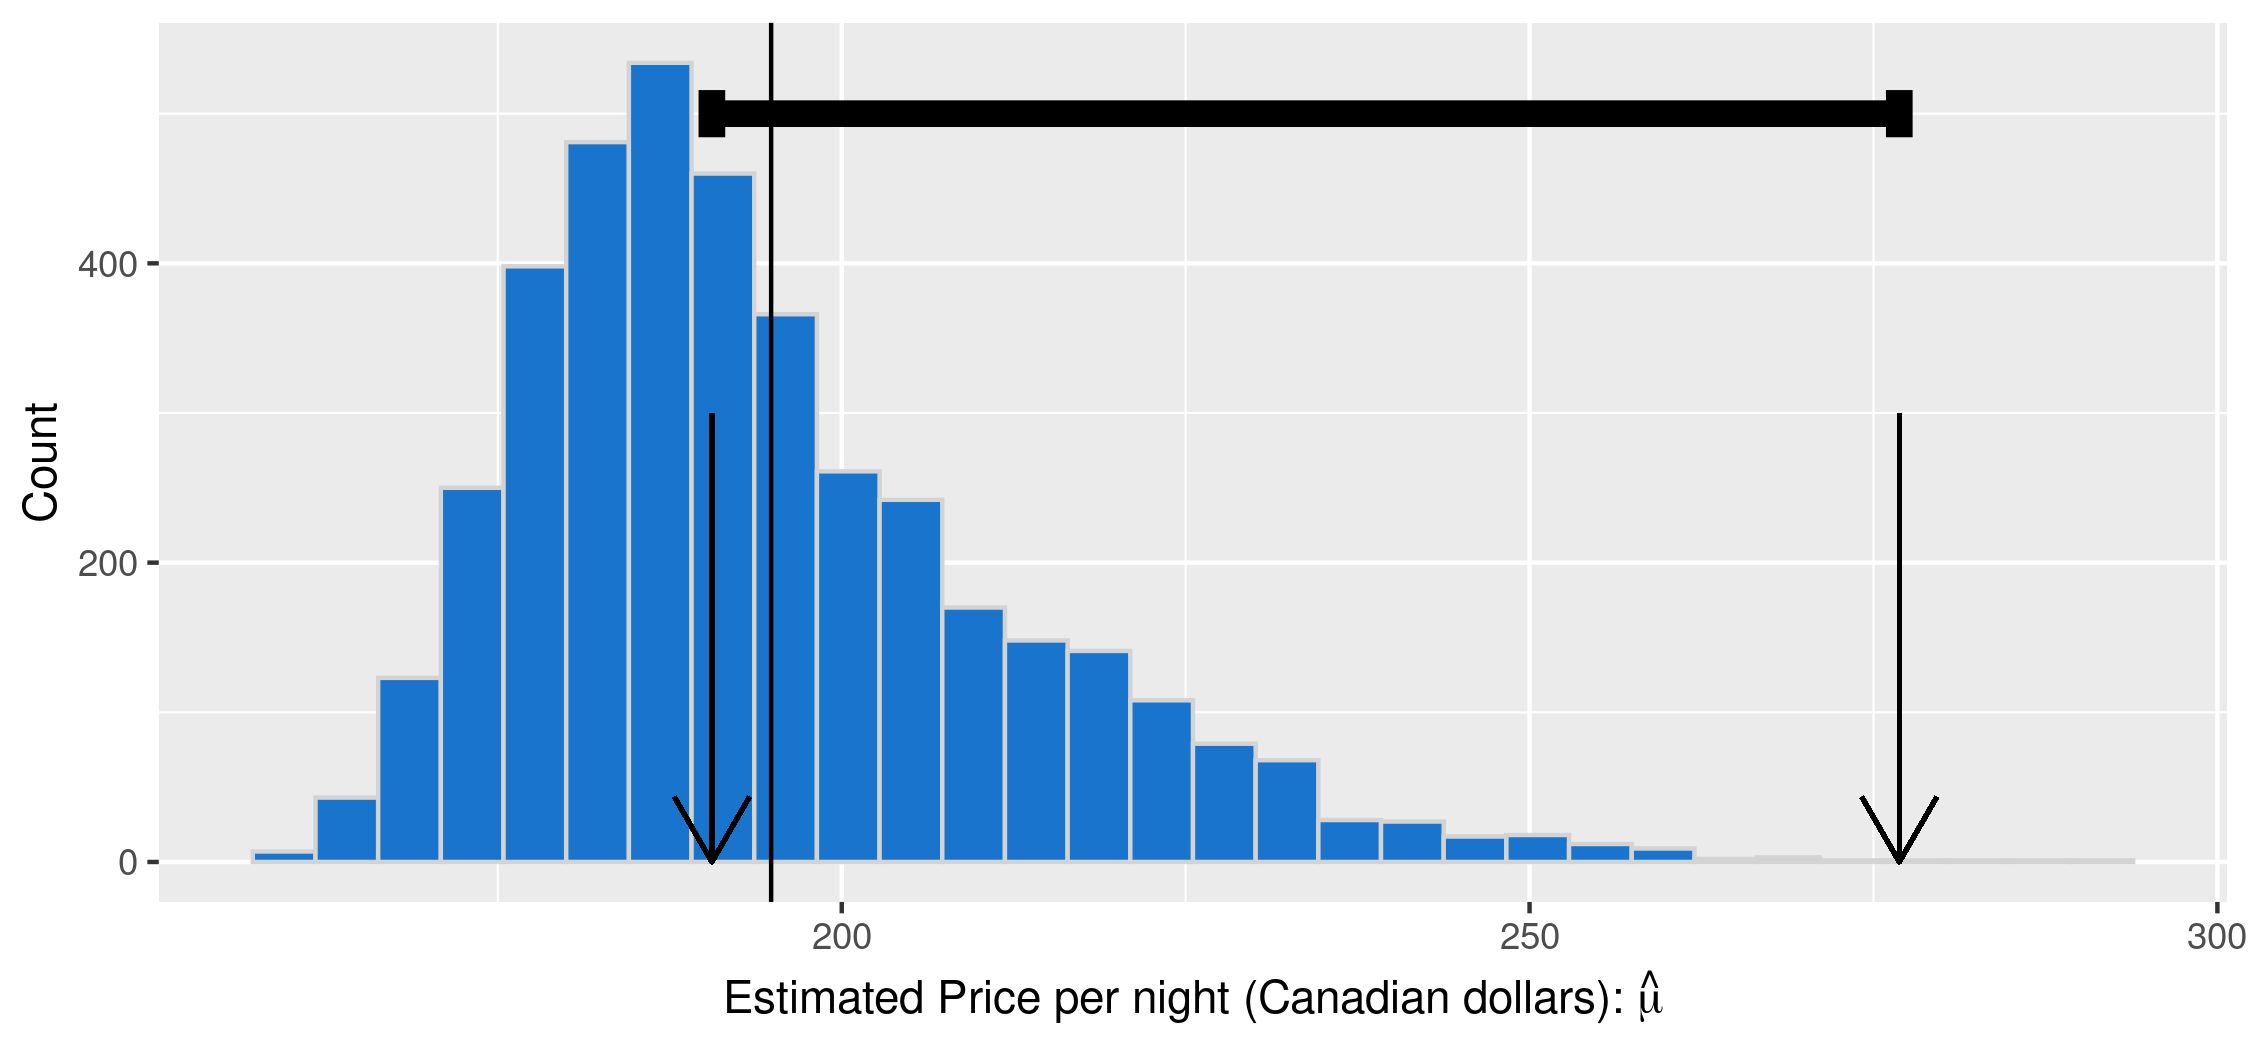
\includegraphics[width=0.98\linewidth,height=0.461\linewidth]{figure/base-hist-ci-1} 

}



\end{knitrout}
}




\newcommand{\SingleCIB}{
\begin{knitrout}
\definecolor{shadecolor}{rgb}{0.969, 0.969, 0.969}\color{fgcolor}

{\centering 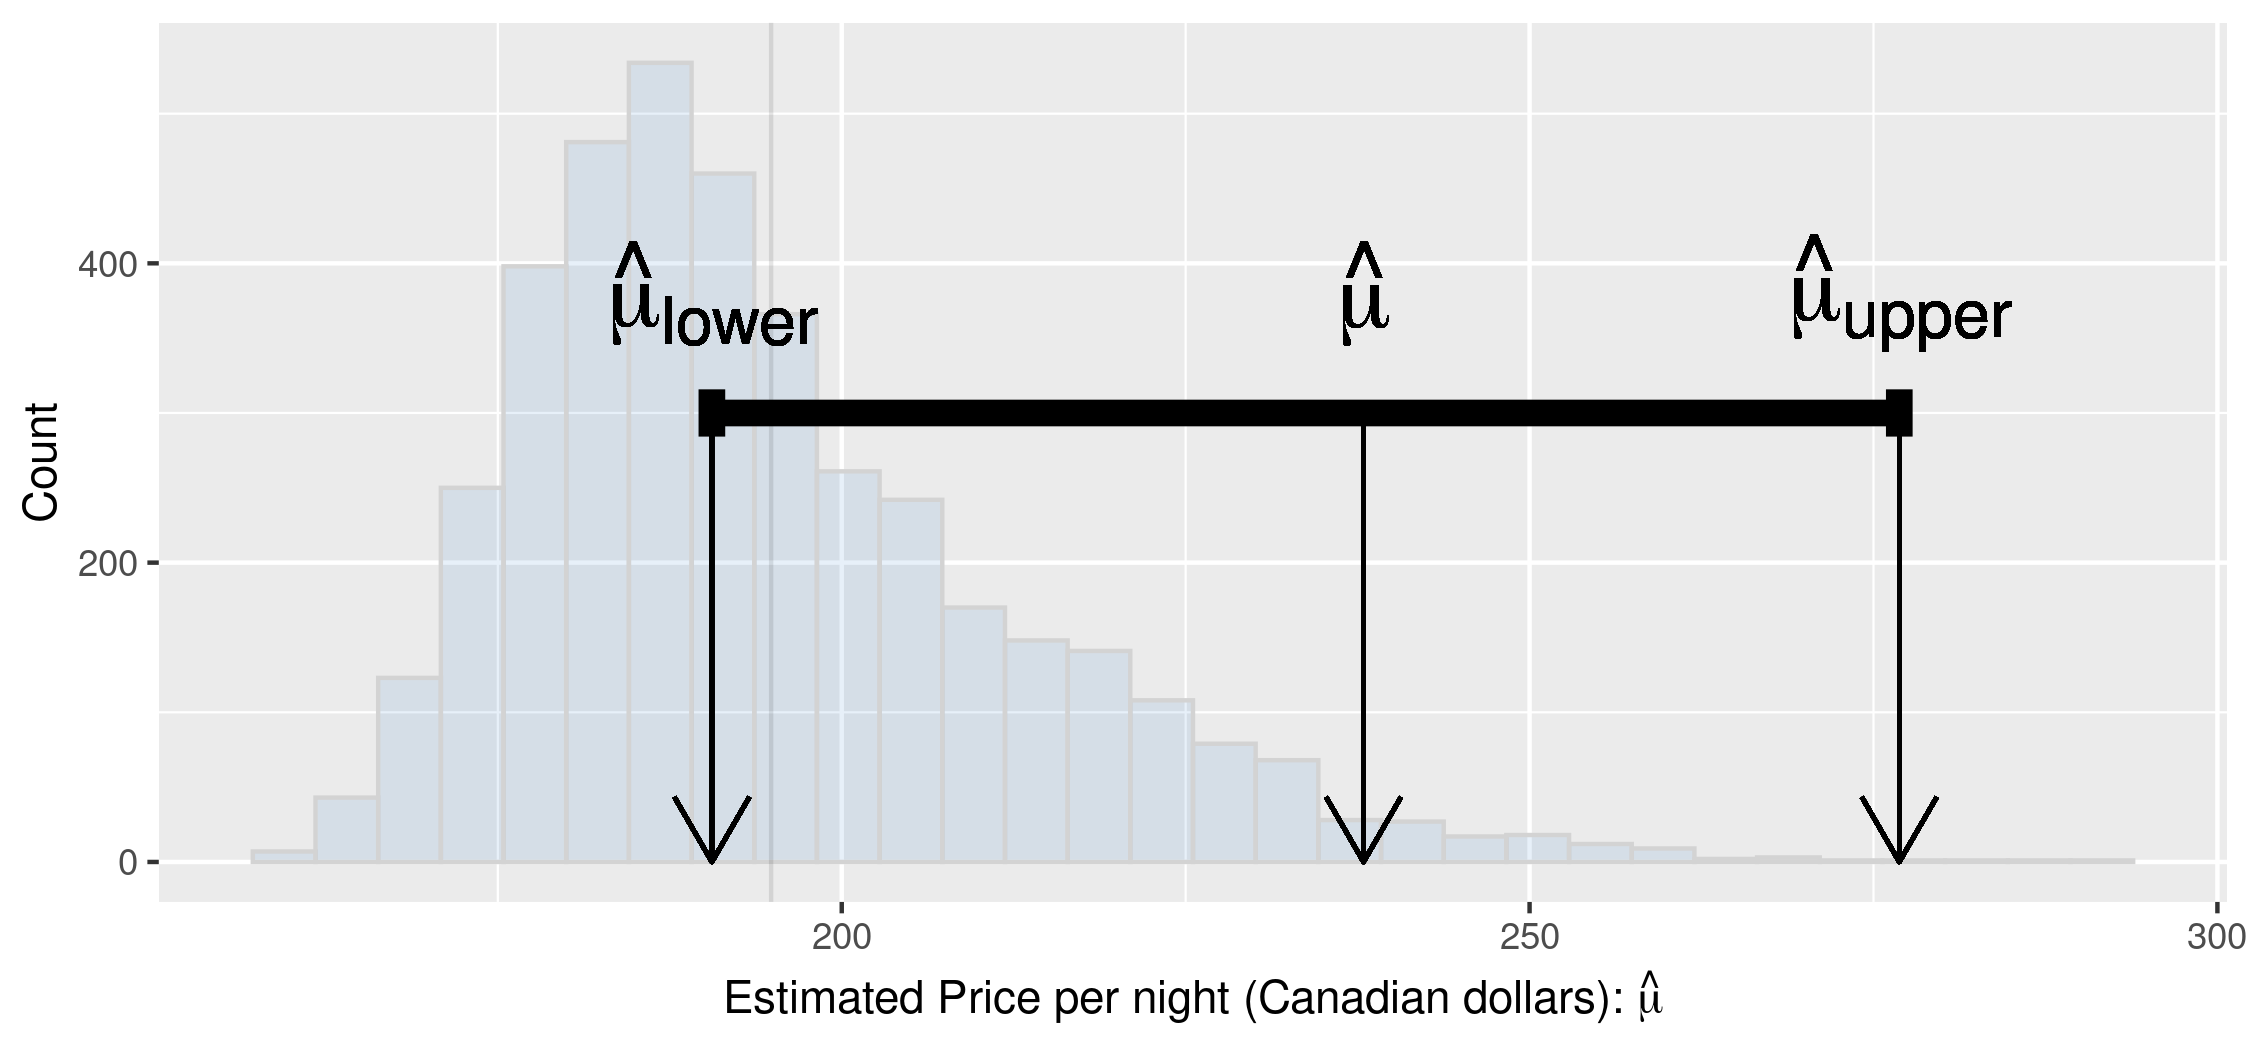
\includegraphics[width=0.98\linewidth,height=0.461\linewidth]{figure/base-hist-cib-1} 

}



\end{knitrout}
}



\newcommand{\MultipleCIs}{



\begin{knitrout}
\definecolor{shadecolor}{rgb}{0.969, 0.969, 0.969}\color{fgcolor}

{\centering 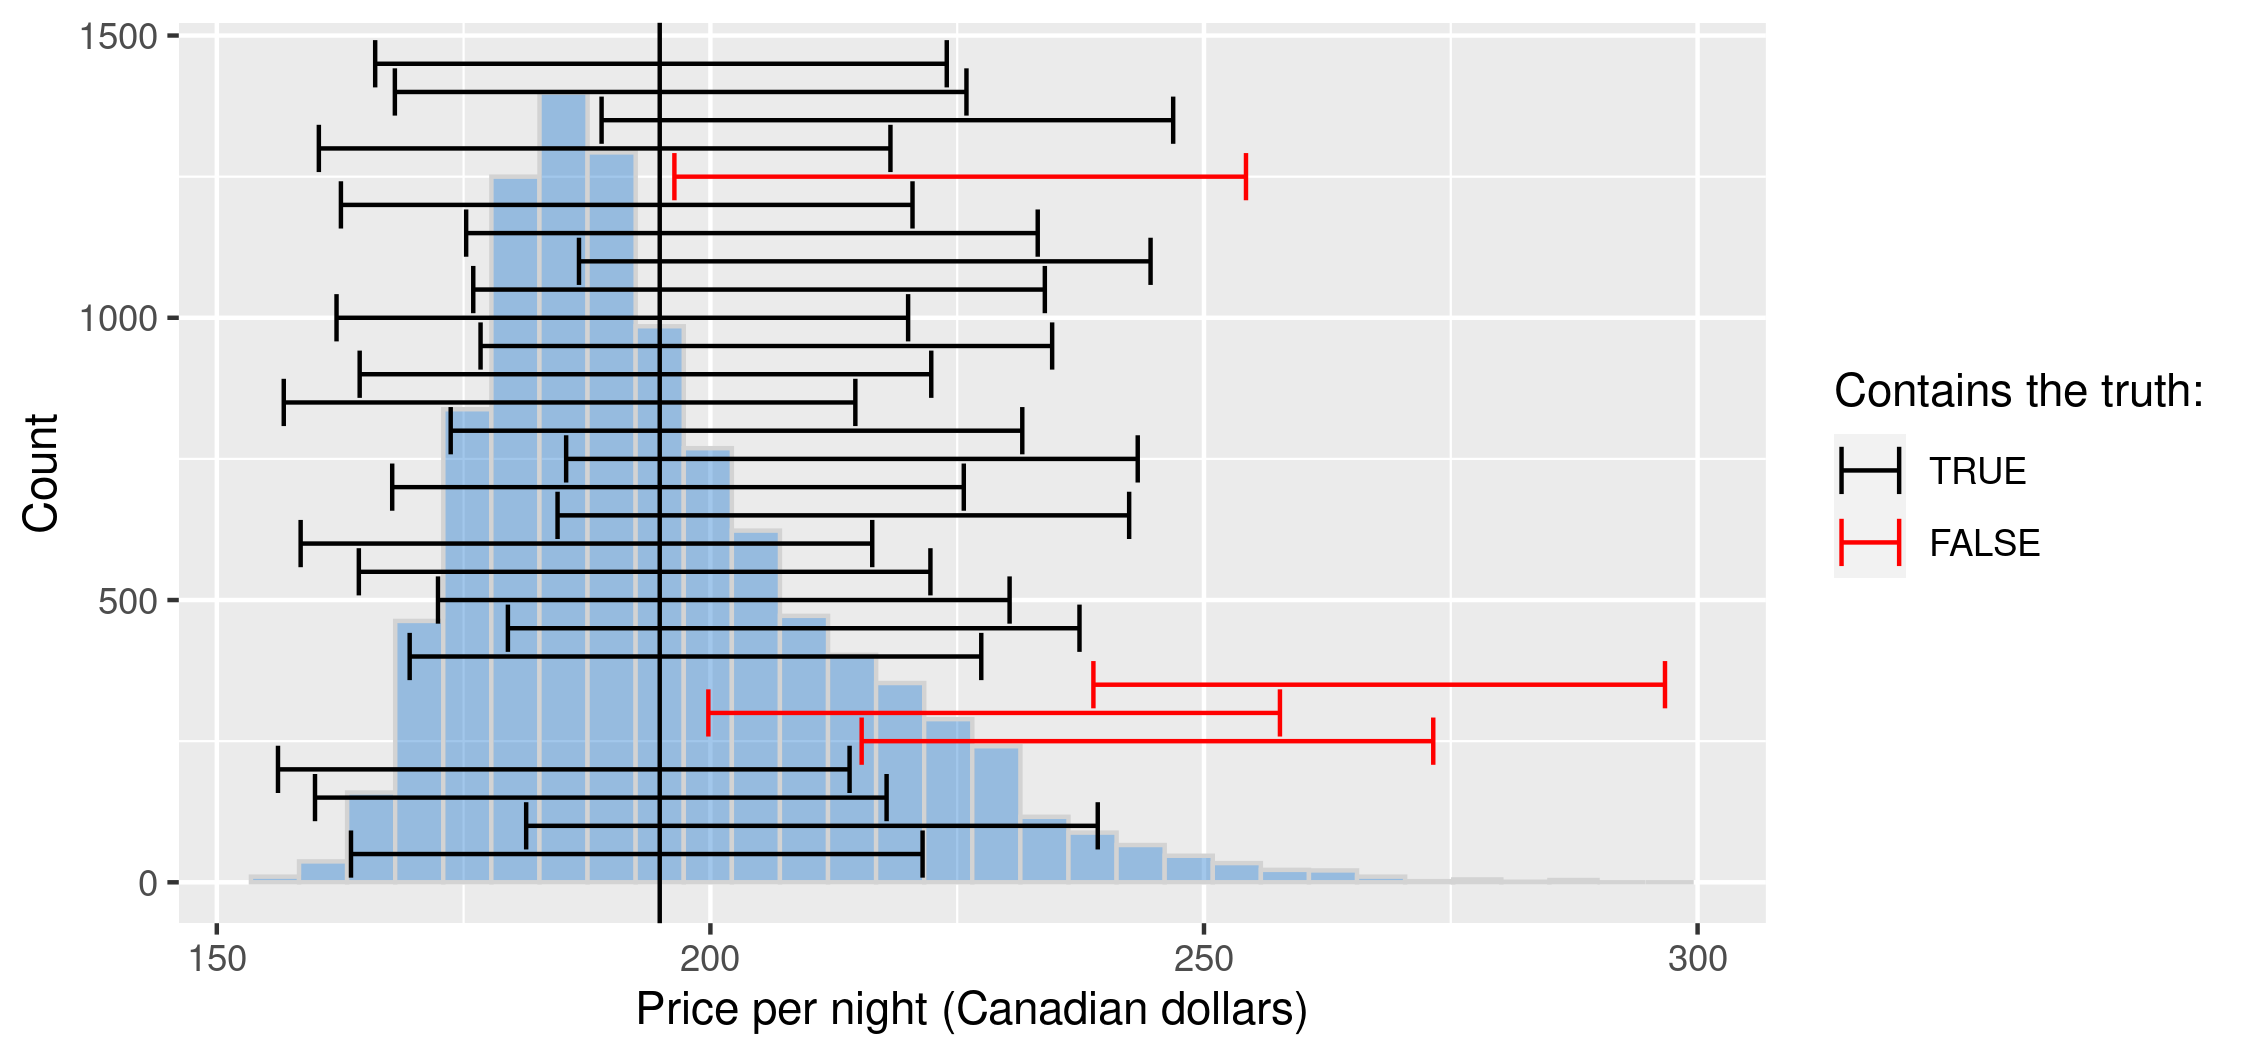
\includegraphics[width=0.98\linewidth,height=0.461\linewidth]{figure/base-hist-cis-1} 

}



\end{knitrout}
}


%%%%%%%%%%%%%%%%%%%%
% amsthm commands

\theoremstyle{plain}
\newtheorem{lem}{Lemma}
\newtheorem{thm}{Theorem}
\newtheorem{prop}{Proposition}
\newtheorem{cond}{Condition}
\newtheorem{assu}{Assumption}
\newtheorem{cor}{Corollary}
\newtheorem{conj}{Conjecture}

\theoremstyle{definition}
\newtheorem{defn}{Definition}
%\newtheorem{ex}{Example}

% Example environment with a terminating symbol.
% https://tex.stackexchange.com/questions/16453/denoting-the-end-of-example-remark
\theoremstyle{definition}
\newtheorem{examplex}{Example}
\newenvironment{ex}
  {\pushQED{\qed}\renewcommand{\qedsymbol}{$\triangle$}\examplex}
  {\popQED\endexamplex}


%%%%%%%%%%%%%%%%%%%%
% refstyle commands

\newref{event}{
    name=Event~, %
    names=Events~, %
    Name=Event~,
    Names=Events~
    }

\newref{item}{
    name=Item~, %
    names=Items~, %
    Name=Item~,
    Names=Items~
    }

\newref{fig}{
    name=Figure~, %
    Name=Figure~
    }

\newref{tab}{
    name=Table~, %
    Name=Table~
    }

\newref{sec}{
    name=Section~, %
    Name=Section~,
    names=Sections~, %
    Names=Sections~
    }

\newref{app}{
    name=Appendix~, %
    Name=Appendix~
    }

\newref{eq}{
    name=Eq.~, %
    Name=Eq.~,
    names=Eqs.~, %
    Names=Eqs.~
    }

\newref{fig}{
    name=Figure~, %
    Name=Figure~
    }

\newref{def}{
    name=Definition~, %
    Name=Definition~
    }

\newref{assu}{
    name=Assumption~, %
    Name=Assumption~,
    names=Assumptions~, %
    Names=Assumptions~,
    }

\newref{cond}{
    name=Condition~, %
    Name=Condition~,
    names=Conditions~, %
    Names=Conditions~
    }

\newref{prop}{
    name=Proposition~, %
    Name=Proposition~,
    names=Propositions~, %
    Names=Propositions~
    }

\newref{lem}{
    name=Lemma~, %
    Name=Lemma~,
    names=Lemmas~, %
    Names=Lemmas~
    }

\newref{ex}{
    name=Example~, %
    Name=Example~}

\newref{cor}{
    name=Corollary~, %
    Name=Corollary~
    }

\newref{thm}{
    name=Theorem~, %
    Name=Theorem~,
    names=Theorems~, %
    Names=Theorems~
    }

\newref{proof}{
    name=Proof~, %
    Name=Proof~
    }

\newref{conj}{
    name=Conjecture~, %
    Name=Conjecture~
    }

\newref{algr}{
    name=Algorithm~, %
    Name=Algorithm~,
    names=Algorithms~, %
    Names=Algorithms~,
    }


%% refstyle examples:
% \Secref[vref]{introduction} contains \secref{introduction}.
% \Secref[vref]{ack} does not contain \secref{introduction}.
%
% \begin{align}
%     x=y \eqlabel{myeq}
% \end{align}
%


\DefineMacros{}

\title{When Can Dropping a Little Data Make a Big Difference?}
\author{Ryan Giordano (\texttt{rgiordan@mit.edu})}
\date{January 2022}
% \institute{University of California, Berkeley}

\setbeamertemplate{Collaborators}[none]
\IfFileExists{upquote.sty}{\usepackage{upquote}}{}
\begin{document}


\begin{frame}{Mister freakin P}


\end{frame}






%%%%%%%%%%%%%%%%%%%%%%%%%%%%%%%%%%%%%%%%%%%%%%%%%%%%%%%%%%%%%%%%%%%%%%%%%%%%
%%%%%%%%%%%%%%%%%%%%%%%%%%%%%%%%%%%%%%%%%%%%%%%%%%%%%%%%%%%%%%%%%%%%%%%%%%%%
%%%%%%%%%%%%%%%%%%%%%%%%%%%%%%%%%%%%%%%%%%%%%%%%%%%%%%%%%%%%%%%%%%%%%%%%%%%%

\begin{frame}[t]{Formalizing the question.}

\begin{minipage}[t]{0.45\textwidth}
\textbf{Ordinary least squares}

A data point $\d_n$ has regressors
$x_n$ and response $y_n$: $\d_n = (x_n, y_n)$.

\vspace{1em}
The estimator $\thetahat \in \mathbb{R}^p$ satisfies:
%
\begin{align*}
%
\thetahat :={}&
    \argmin_{\theta} \frac{1}{2} \sumn \left(y_n - \theta^T x_n \right)^{2} \\
\Leftrightarrow{}& \sumn \left(y_n - \thetahat^T x_n \right) x_n = 0.
%
\end{align*}
%
Make a qualitative decision using:\vspace{-1.5em}
\begin{itemize}
\item A particular component: $\theta_k$
\item The end of a confidence interval:
    $\theta_k + \frac{1.96}{\sqrt{N}} \hat\sigma(\thetahat)$
\end{itemize}
%
\end{minipage}
%
\hfill\vline\hfill
%
\begin{minipage}[t]{0.45\textwidth}
\textbf{Z-estimators}

We observe $N$ data points $\d_{1}, \ldots, \d_{N}$
(in any domain).

\vspace{1em}
The estimator $\thetahat \in \mathbb{R}^p$ satisfies:
%
\begin{align*}
%
\sumn
G(\thetahat, \d_{n}) =  \zP.
%
\end{align*}
%
$G(\cdot, \d_{n})$ is ``nice,'' $\mathbb{R}^p$-valued.

E.g. OLS, MLE, VB, IV \&c.

\vspace{1em}
Make a qualitative decision using $\thetafun(\thetahat)$
for a smooth, real-valued $\thetafun$.
%
\end{minipage}

\hrulefill

\vspace{0.3em}
\textbf{Question: }
Can we make a big change in $\thetafun(\thetahat)$ by dropping
$\alphan$ datapoints, for some small proportion $\alpha$?



\end{frame}





%%%%%%%%%%%%%%%%%%%%%%%%%%%%%%%%%%%%%%%%%%%%%%%%%%%%%%%%%%%%%%%%%%%%%%%%%%%%
%%%%%%%%%%%%%%%%%%%%%%%%%%%%%%%%%%%%%%%%%%%%%%%%%%%%%%%%%%%%%%%%%%%%%%%%%%%%
%%%%%%%%%%%%%%%%%%%%%%%%%%%%%%%%%%%%%%%%%%%%%%%%%%%%%%%%%%%%%%%%%%%%%%%%%%%%

\begin{frame}[t]{Which estimators do we study?}

We have $N$ data points $\d_{1}, \ldots, \d_{N}$, a quantity of interest
$\thetafun(\thetahat)$, and
%
\begin{align*}
%
\sumn G(\thetahat, \d_{n}) =  \zP .
%
\end{align*}

\textbf{Question: }
Can we make a big change in $\thetafun(\thetahat)$ by dropping
$\alphan$ datapoints, for some small proportion $\alpha$?
%
\textbf{Two big problems:}
%
\begin{itemize}
    \item There are ${N \choose \alphan}$
        sets to check. (Huge even for $\alpha \ll 1$.)
    \item Evaluating $\thetahat$ re-solving the estimating equation.
        \begin{itemize}
        \item E.g., re-computing the OLS estimator.
        \item Other examples are even harder (VB, machine learning)
        \end{itemize}
\end{itemize}
%
\textbf{An approximation is needed!}
\end{frame}



%%%%%%%%%%%%%%%%%%%%%%%%%%%%%%%%%%%%%%%%%%%%%%%%%%%%%%%%%%%%%%%%%%%%%%%%%%%%
%%%%%%%%%%%%%%%%%%%%%%%%%%%%%%%%%%%%%%%%%%%%%%%%%%%%%%%%%%%%%%%%%%%%%%%%%%%%
%%%%%%%%%%%%%%%%%%%%%%%%%%%%%%%%%%%%%%%%%%%%%%%%%%%%%%%%%%%%%%%%%%%%%%%%%%%%

\begin{frame}[t]{Which estimators do we study?}
% Suppose we have $N$ data points $\d_{1}, \ldots, \d_{N}$.  Then:
%
\begin{align*}
%
\thetahat \only<2->{\color{red} (\w) \color{black}} :=
\vec\theta \,\, \textrm{ such that } \,\,
\sumn
\only<2->{ \color{red} \w_{n} \color{black}}
G(\vec\theta, \d_{n}) =  \zP .
%
\end{align*}
%
\begin{minipage}{0.45\textwidth}
\begin{center}
Original weights: $\onevec = (1,\ldots,1)$
    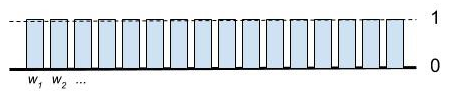
\includegraphics[width=1.0\textwidth]{static_figures/orig_weights}
Leave points out by setting their elements of $\w$ to zero.
    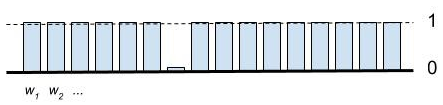
\includegraphics[width=1.0\textwidth]{static_figures/weights_loo}
\end{center}
\end{minipage}
\begin{minipage}{0.45\textwidth}
\begin{center}
    \begin{tikzpicture}
        \node[anchor=south west,inner sep=0] (image) at (0,0) {
            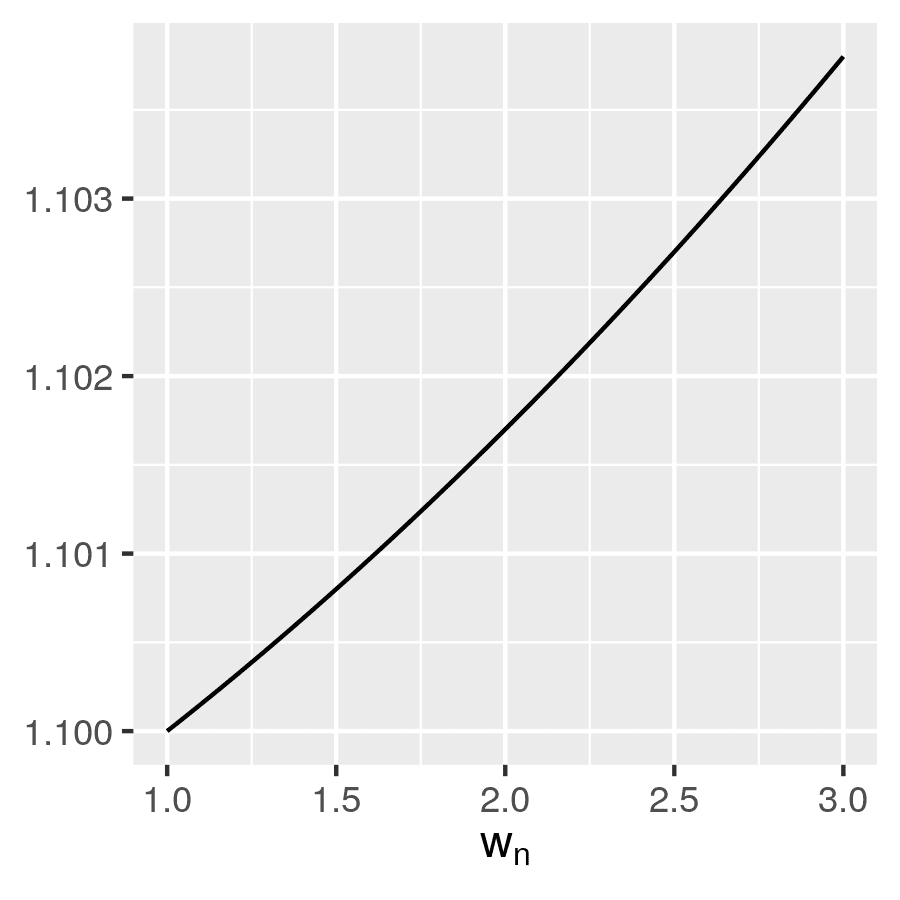
\includegraphics[width=0.88\textwidth]{static_figures/e_beta_w}
        };
        \begin{scope}[x={(image.south east)},y={(image.north west)}]
            \draw[blue, thick, <-] (0.2,0.23) -- ++(0.1,0.25)
                    node[above,black,fill=white]
                    {\small $\thetafun(\thetahat(\onevec))$};
            \draw[blue, thick, <-] (0.8,0.8) -- ++(-0.1,0.1)
                    node[left,black,fill=white]
                    {\small $\thetafun(\thetahat(\w))$};
            \draw[red, thick, -] (0.18,0.18) -- ++(1.2 * 0.6, 1.2 * 0.48);
            \draw[blue, thick, <-] (0.75,0.55) -- ++(0.02,-0.1)
                    node[below,black,fill=white]
                    {\small Slope $ = \infl_n$};
        \end{scope}
    \end{tikzpicture}
\end{center}
\end{minipage}

The slopes $\infl_n := \fracat{\partial \thetafun(\thetahat(\w))}{\partial \w_n}{\onevec}$ are values of the \textbf{empirical influence function}
\citep{hampel1986robustbook}.  We call them ``influence scores.''

% \vspace{1em}
% $\thetahat(\w)$ well-defined even for continuous values of the weights!

\vspace{1em}
Second-order derivatives control the error of
the linear approximation.

\end{frame}




%%%%%%%%%%%%%%%%%%%%%%%%%%%%%%%%%%%%%%%%%%%%%%%%%%%%%%%%%%%%%%%%%%%%%%%%%%%%
%%%%%%%%%%%%%%%%%%%%%%%%%%%%%%%%%%%%%%%%%%%%%%%%%%%%%%%%%%%%%%%%%%%%%%%%%%%%
%%%%%%%%%%%%%%%%%%%%%%%%%%%%%%%%%%%%%%%%%%%%%%%%%%%%%%%%%%%%%%%%%%%%%%%%%%%%


\begin{frame}{Taylor series approximation.}
%
\textbf{Problem: } How large can you make $\thetafun(\thetahat(\w))$
leaving out no more than $\alphan$ points?  \textbf{Combinatorially hard!}

\hrulefill

\vspace{1em}
To simplify the search over $\w$, we form the Taylor series approximation:
%
\begin{align*}
	\thetafun(\thetahat(\w))
		&\approx
        \color{red}
        \thetafunlin(\w)
        \color{black}
		:=  \thetafun(\thetahat(\onevec)) +
        \sumn \infl_n (\w_n -1)
        \color{black}
\end{align*}
%
\textbf{Approximate solution: } How large can you make $\thetafunlin(\w)$
leaving out no more than $\alphan$ points?  \textbf{Easy! }

\vspace{1em}
The most influential points for $\thetafunlin(\w)$ have the
most negative $\infl_n$.

\hrulefill

The $\infl_n$ are automatically computable using the
\textbf{implicit function theorem} and \textbf{automatic differentiation}.

\hrulefill

We provide \textbf{finite-sample theory} showing that
$\abs{\thetafun(\thetahat(\w)) - \thetafunlin(\w)} =
O\left(\vnorm{\frac{1}{N}(\w - \onevec)}^2_2\right) =
O\left(\alpha\right)$ as $\alpha \rightarrow 0$.

\end{frame}


%
% %%%%%%%%%%%%%%%%%%%%%%%%%%%%%%%%%%%%%%%%%%%%%%%%%%%%%%%%%%%%%%%%%%%%%%%
% %%%%%%%%%%%%%%%%%%%%%%%%%%%%%%%%%%%%%%%%%%%%%%%%%%%%%%%%%%%%%%%%%%%%%%%
% %%%%%%%%%%%%%%%%%%%%%%%%%%%%%%%%%%%%%%%%%%%%%%%%%%%%%%%%%%%%%%%%%%%%%%%
%
% \begin{frame}{Taylor series approximation.}
%
% \vspace{1em}
% \textbf{How to compute the influence scores $\infl_n$? }
%
%
% By the chain rule,
% $\infl_n = \fracat{\partial \thetafun(\thetahat(\w))}{\partial \w_n}{\onevec}
% = \fracat{\dee \thetafun(\theta)}
%     {\dee \theta^T}{\thetahat}
%   \fracat{\partial \thetahat(\w)}{\partial \w_n}{\onevec}$.
%
% Recall that
% %\begin{align*}
% %
% $\thetahat(\w) :=
% \vec\theta \,\, \textrm{ such that } \,\,
% \sumn \w_{n}  G(\vec\theta, \d_{n}) =  \zP$.
% %
% %\end{align*}
% %
%
% The \textbf{implicit function theorem} expresses $\fracat{\partial
% \thetahat(\w)}{\partial \w_n}{\onevec}$ as a linear system.
%
% \vspace{1em}
% Computation of $\infl_n$ is fully automatible from a
% software implemenation of $G(\cdot, \cdot)$ and $\thetafun(\cdot)$ with
% \textbf{automatic differentiation}
% \citep{baydin2017automatic}.
%
% \vspace{1em}
% We have an \texttt{R} package, \texttt{rgiordan/zaminfluence},
% for OLS and IV.
%
% \end{frame}



%%%%%%%%%%%%%%%%%%%%%%%%%%%%%%%%%%%%%%%%%%%%%%%%%%%%%%%%%%%%%%%%%%%%%%%%%%%%
%%%%%%%%%%%%%%%%%%%%%%%%%%%%%%%%%%%%%%%%%%%%%%%%%%%%%%%%%%%%%%%%%%%%%%%%%%%%
%%%%%%%%%%%%%%%%%%%%%%%%%%%%%%%%%%%%%%%%%%%%%%%%%%%%%%%%%%%%%%%%%%%%%%%%%%%%


\begin{frame}{Taylor series approximation.}

\textbf{Procedure:}

\begin{enumerate}
    \item<2-> Compute the ``original'' estimator, $\thetahat(\onevec)$ and
    $\thetafun(\thetahat(\onevec))$.
    \item<3-> Let $\Delta$ denote an increase in $\thetafun(\thetahat)$
    that would change conclusions.
    % if there is
    % a $\w^*$ with no more than $\alphan$ zeros such that
    %
    % \begin{align*}
    % %
    % \thetafun(\thetahat(\w^*)) - \thetafun(\thetahat(\onevec)) \ge \Delta
    % %
    % \end{align*}
    %
    \item<4-> Compute and sort the influence scores,
        $\infl_{(1)} \le \infl_{(2)} \le \ldots \le \infl_{(N)}$.
    \item<5-> Let $\w^*$ leave out the data corresponding to
    $\infl_{(1)},  \ldots , \infl_{(\alphan)}$.
    %the $\lfloor \alpha N \rfloor$ most negative influence scores.
    \item<6-> Report non-robustness if
        $ \thetafunlin(\w^*) - \thetafun(\thetahat)  =
            - \sum_{n=1}^{\alphan} \infl_{(n)} \ge \Delta$.
    \item<7-> \textbf{Optional: } Compute $\thetahat(\w^*)$, and verify
    that $\thetafun(\thetahat(\w^*)) - \thetafun(\thetahat) \ge \Delta$.
\end{enumerate}

\end{frame}



%%%%%%%%%%%%%%%%%%%%%%%%%%%%%%%%%%%%%%%%%%%%%%%%%%%%%%%%%%%%%%%%%%%%%%%%%
%%%%%%%%%%%%%%%%%%%%%%%%%%%%%%%%%%%%%%%%%%%%%%%%%%%%%%%%%%%%%%%%%%%%%%%%%
%%%%%%%%%%%%%%%%%%%%%%%%%%%%%%%%%%%%%%%%%%%%%%%%%%%%%%%%%%%%%%%%%%%%%%%%%

% \begin{frame}{The linear approximation.}
%
% For $N=\SimNumObs$ data points, compute the OLS estimator from:
%
% \vspace{1em}
% \begin{tabularx}{\textwidth}{YYY}
% %\begin{tabular}{ccc}
%     Regressors  &   Residuals   &   Responses \\
%     $x_n \sim \mathcal{N}(0, \sigma_x^2)$   &
%     $\varepsilon_n \sim \mathcal{N}(0, \sigma_\varepsilon^2)$   &
%     $y_n = \theta_0 x_n + \varepsilon_n$
% \end{tabularx}
% %
%
% \SimApproxNormalGraph{}
%
% \end{frame}


%%%%%%%%%%%%%%%%%%%%%%%%%%%%%%%%%%%%%%%%%%%%%%%%%%%%%%%%%%%%%%%%%%%%%%%%%
%%%%%%%%%%%%%%%%%%%%%%%%%%%%%%%%%%%%%%%%%%%%%%%%%%%%%%%%%%%%%%%%%%%%%%%%%
%%%%%%%%%%%%%%%%%%%%%%%%%%%%%%%%%%%%%%%%%%%%%%%%%%%%%%%%%%%%%%%%%%%%%%%%%


\begin{frame}


Mexico example:

See \texttt{microcredit\_profit\_sandbox.R}.

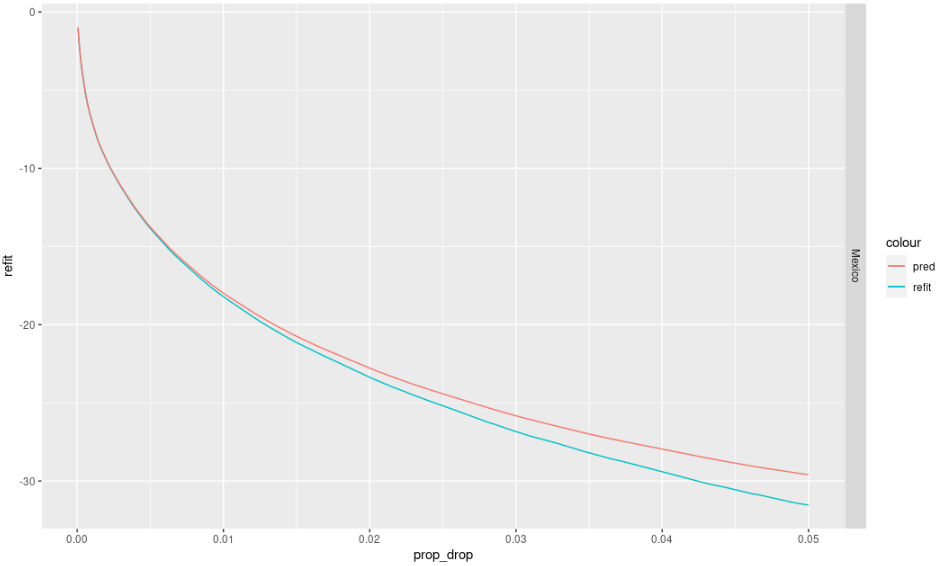
\includegraphics[width=0.9\textwidth]{static_figures/mx_refit_example}

\end{frame}





%%%%%%%%%%%%%%%%%%%%%%%%%%%%%%%%%%%%%%%%%%%%%%%%%%%%%%%%%%%%%%%%%%%%%%%%%
%%%%%%%%%%%%%%%%%%%%%%%%%%%%%%%%%%%%%%%%%%%%%%%%%%%%%%%%%%%%%%%%%%%%%%%%%
%%%%%%%%%%%%%%%%%%%%%%%%%%%%%%%%%%%%%%%%%%%%%%%%%%%%%%%%%%%%%%%%%%%%%%%%%

\begin{frame}{Selected experimental results.}

\begin{itemize}
\item The ``Refit estimate'' column shows the result of re-fitting the model removing
the points with the largest influence scores.

\item Stars indicate significance at the 5\% level.

\item Refits that achieved the desired change are bolded.
\end{itemize}

{
\footnotesize
\MicrocreditProfitResultsTable{}
}

\onslide<2->{
\footnotesize
\CashTransfersResultsTable{}
}

\end{frame}



%%%%%%%%%%%%%%%%%%%%%%%%%%%%%%%%%%%%%%%%%%%%%%%%%%%%%%%%%%%%%%%%%%%%%%%%%
%%%%%%%%%%%%%%%%%%%%%%%%%%%%%%%%%%%%%%%%%%%%%%%%%%%%%%%%%%%%%%%%%%%%%%%%%
%%%%%%%%%%%%%%%%%%%%%%%%%%%%%%%%%%%%%%%%%%%%%%%%%%%%%%%%%%%%%%%%%%%%%%%%%


\begin{frame}{A simulation}

For $N=\SimNumObs$ data points, compute the OLS estimator from:

\vspace{1em}
\begin{tabularx}{\textwidth}{YYY}
%\begin{tabular}{ccc}
    Regressors  &   Residuals   &   Responses \\
    $x_n \sim \mathcal{N}(0, \sigma_x^2)$   &
    $\varepsilon_n \sim \mathcal{N}(0, \sigma_\varepsilon^2)$   &
    $y_n = \SimTrueTheta x_n + \varepsilon_n$
\end{tabularx}
%

\SimGridNormalGraph{}

\end{frame}







%%%%%%%%%%%%%%%%%%%%%%%%%%%%%%%%%%%%%%%%%%%%%%%%%%%%%%%%%%%%%%%%%%%%%%%%%
%%%%%%%%%%%%%%%%%%%%%%%%%%%%%%%%%%%%%%%%%%%%%%%%%%%%%%%%%%%%%%%%%%%%%%%%%
%%%%%%%%%%%%%%%%%%%%%%%%%%%%%%%%%%%%%%%%%%%%%%%%%%%%%%%%%%%%%%%%%%%%%%%%%

\begin{frame}{What makes an analysis sensitive?  Preliminaries}
%
We are \textbf{robust to data dropping} if, for the $\Delta$
that changes conclusions and $\w^*$ dropping the $\alphan$
most influential points,
%
\begin{align*}
% $
%
\Delta \ge \thetafunlin(\w^*) - \thetafun(\thetahat(\onevec))
    % = {\color{red}- \sum_{n=1}^{\lfloor \alpha N \rfloor} \infl_{(n)} }
    =:   {\color{black} \noise } { \color{black} \shape}
\quad\Leftrightarrow\quad
%
{\color{red}\frac{\Delta}{\noise} \ge \shape}.
%
% $
\end{align*}
%
% \hspace{1em} where \vspace{1em}

\begin{itemize}
\item The ``signal'' $\Delta$ is the smallest change that reverses your conclusion
\item The ``noise'' $\noise^2 \rightarrow \mathrm{Var}(\sqrt{N}\phi)$
    (``sandwich'' variance estimator)
\item The ``shape''
    $\shape$
    $\rightarrow$ a nonzero constant and is
    $\le \sqrt{\alpha (1 - \alpha)}$
\end{itemize}

\hrulefill

\textbf{Contrast with sampling variability.}

A 95\% CI is given by
$\thetafun(\thetahat(\onevec)) \pm \frac{1.96}{\sqrt{N}} \noise.$
%
We reject $\thetafun(\thetahat(\onevec)) + \Delta$ when
%
\begin{align*}
%
\thetafun(\thetahat(\onevec)) + \Delta \ge
\thetafun(\thetahat(\onevec)) + \frac{1.96}{\sqrt{N}} \noise
\quad\quad
\Leftrightarrow
\quad\quad
{\color{red}
\frac{\Delta}{\noise} \ge \frac{1.96}{\sqrt{N}.}
}
%
\end{align*}
%


\hrulefill

%\vspace{1em}
The \textbf{signal to noise ratio} $\frac{\Delta}{\noise}$
determines robustness to both data dropping
and sampling variability, but with \textbf{different thresholds}.

% \begin{center}
% \begin{minipage}{0.8\textwidth}
% \begin{tikzpicture}
%     \node[anchor=south west,inner sep=0] (image) at (0,0) {
%     \SimInflHistogram{}
%     };
%     \begin{scope}[x={(image.south east)},y={(image.north west)}]
%         \draw [stealth-stealth][thick][white](0.42, 0.35) -- (0.6, 0.35);
%         \draw (0.51, 0.35) node[below][text width=3cm][align=center][white]
%             {\normalsize $\noise$};
%
%         \draw [stealth-][thick][red](0.3, 0.25) -- (0.3, 0.5);
%         \draw (0.25, 0.5) node[above][text width=3cm][align=center][red]
%             {\normalsize $-\sum_{n=1}^{\alphan} \infl_{(n)}$};
%     \end{scope}
% \end{tikzpicture}
% \end{minipage}
% \end{center}

\end{frame}



%%%%%%%%%%%%%%%%%%%%%%%%%%%%%%%%%%%%%%%%%%%%%%%%%%%%%%%%%%%%%%%%%%%%%%%%%
%%%%%%%%%%%%%%%%%%%%%%%%%%%%%%%%%%%%%%%%%%%%%%%%%%%%%%%%%%%%%%%%%%%%%%%%%
%%%%%%%%%%%%%%%%%%%%%%%%%%%%%%%%%%%%%%%%%%%%%%%%%%%%%%%%%%%%%%%%%%%%%%%%%

\begin{frame}[t]{What makes an analysis sensitive?}
%
\begin{minipage}{0.45\textwidth}
\begin{center}
    Robust to data dropping:\\
    (``dropping robustness'')\\
    \vspace{1em}
    $\textrm{SNR} := \frac{\Delta}{\noise} \ge \shape$
\end{center}
\end{minipage}
%
\begin{minipage}{0.45\textwidth}
\begin{center}
    Robust to sampling variation:\\
    (``sampling robustness'')\\
    \vspace{1em}
    $\textrm{SNR} := \frac{\Delta}{\noise} \ge
        \frac{1.96}{\sqrt{N}}$
\end{center}
\end{minipage}

\vspace{1em}

\hrulefill

\vspace{0.5em} $\bullet\quad$
\textbf{Dropping robustness $\ne$ sampling robustness in general.\\}
\textit{Proof: }
$\shape \ne \frac{1.96}{\sqrt{N}}$.

\vspace{0.5em} $\bullet\quad$
\textbf{When the SNR is small, sufficiently large $N$
produces sampling robustness, but not necessarily
dropping robustness.\\}
\textit{Proof: }
$\frac{1.96}{\sqrt{N}} \rightarrow 0$, but $\shape \rightarrow$ a nonzero
constant.

\vspace{0.5em} $\bullet\quad$
\textbf{Statistical insignificance is dropping non-robust for large $N$.\\}
\textit{Proof: }
%
Insignificance means
$|\thetafun(\thetahat(\onevec))| \le \frac{1.96}{\sqrt{N}} \noise$.

$\Rightarrow$ A result can be made significant by a change of no more than
$\frac{1.96}{\sqrt{N}} \noise$.

$\Rightarrow$ The SNR for a conclusion
of ``insignificance'' is $\frac{\Delta}{\noise} \le \frac{1.96}{\sqrt{N}}
\rightarrow 0 \le \shape$.

\vspace{0.5em} $\bullet\quad$
\textbf{P-hacking is dropping non-robust for large $N$.\\}
\textit{Proof: }P-hacked effect sizes are of the order
$\frac{1.96}{\sqrt{N}} \noise$.

\end{frame}



%%%%%%%%%%%%%%%%%%%%%%%%%%%%%%%%%%%%%%%%%%%%%%%%%%%%%%%%%%%%%%%%%%%%%%%%%
%%%%%%%%%%%%%%%%%%%%%%%%%%%%%%%%%%%%%%%%%%%%%%%%%%%%%%%%%%%%%%%%%%%%%%%%%
%%%%%%%%%%%%%%%%%%%%%%%%%%%%%%%%%%%%%%%%%%%%%%%%%%%%%%%%%%%%%%%%%%%%%%%%%

\begin{frame}[t]{What makes an analysis sensitive?}
%
\begin{minipage}[t]{0.45\textwidth}
\begin{center}
    Robust to data dropping:\\
    (``dropping robustness'')\\
    \vspace{1em}
    $\textrm{SNR} := \frac{\Delta}{\noise} \ge \shape$
\end{center}
\end{minipage}
%
\begin{minipage}[t]{0.45\textwidth}
\begin{center}
    Robust to gross errors:\\
    (``gross error robustness'')\\
    \vspace{1em}
    Gross outliers cannot produce
    arbitrarily large changes to $\thetafun$.
\end{center}
\end{minipage}

\vspace{1em}
\hrulefill

\vspace{1em} $\bullet\quad$
\textbf{Dropping non-robustness is not driven by misspecification.\\}
\textit{Proof: }
Small $\Delta$ are dropping non-robust irrespective of specification.

\vspace{1em} $\bullet\quad$
\textbf{Gross outliers primarily affect dropping robustness through $\noise$.\\}
\textit{Proof: }
For a fixed $\noise$, outliers decrease $\shape$.
(Details in paper.)

\end{frame}




%%%%%%%%%%%%%%%%%%%%%%%%%%%%%%%%%%%%%%%%%%%%%%%%%%%%%%%%%%%%%%%%%%%%%%%%%
%%%%%%%%%%%%%%%%%%%%%%%%%%%%%%%%%%%%%%%%%%%%%%%%%%%%%%%%%%%%%%%%%%%%%%%%%
%%%%%%%%%%%%%%%%%%%%%%%%%%%%%%%%%%%%%%%%%%%%%%%%%%%%%%%%%%%%%%%%%%%%%%%%%

\begin{frame}[t]{How to make an analysis less sensitive?}

\begin{center}
    Robust to data dropping:\\
    (``dropping robustness'')\\
    \vspace{1em}
    $\textrm{SNR} := \frac{\Delta}{\noise} \ge \shape$
\end{center}

\vspace{1em}
\hrulefill

\vspace{1em}
\textbf{To achieve dropping robustness,
reduce $\noise$ and / or increase $\Delta$.\\}
\textit{Proof: }
Across typical distributions, $\shape$ varies little.
(Details in paper.)

% \vspace{1em}
% \hrulefill

\vspace{1em}
In the Mexico microcredit example,
%
\begin{align*}
%
\noise = \MxNoise
\quad\quad\quad
\thetafun(\thetahat(\onevec)) = \MxBetahat
\quad\quad\quad
N = \MxNobs
%
\end{align*}
%
The study overcame a very low signal to noise ratio with a very large $N$.

\vspace{1em} This (canonical) response to low signal to noise ratio --- to
gather more data --- produces small SEs, but cannot produce dropping
robustness.

\end{frame}


\begin{frame}{Conclusion}

\begin{itemize}
%
\item Variational inference can be thought of as \emph{approximate marginalization using optimization}.
%
\item Not only is variational inference closely related to familiar existing
frequentist methods (like the EM algorithm), it can help us understand those
methods better.
%
\item The key to a good variational approximation is \emph{tractable
expectations}, \emph{tractable entropy}, and \emph{expressivity}.
%
\item It is important to be aware of variational inference's shortcomings (e.g.,
underestimation of variance in the mean field approximation).
%
\item There are a zillion topics to work on in variational inference.
A good place to start reading is \citet{blei2017variational}.
%
\end{itemize}

\begin{center}
    \textbf{Thanks for having me!}
\end{center}

\end{frame}



\begin{frame}{}
\begin{center}
    {\Huge \textbf{Extra slides}}
\end{center}
\end{frame}


%%%%%%%%%%%%%%%%%%%%%%%%%%%%%%%%%%%%%%%%%%%%%%%%%%%%%%%%%%%%%%%%%%%%%%%%%
%%%%%%%%%%%%%%%%%%%%%%%%%%%%%%%%%%%%%%%%%%%%%%%%%%%%%%%%%%%%%%%%%%%%%%%%%
%%%%%%%%%%%%%%%%%%%%%%%%%%%%%%%%%%%%%%%%%%%%%%%%%%%%%%%%%%%%%%%%%%%%%%%%%


\begin{frame}{A simulation}

For $N=\SimNumObs$ data points, compute the OLS estimator from:

\vspace{1em}
\begin{tabularx}{\textwidth}{YYY}
%\begin{tabular}{ccc}
    Regressors  &   Residuals   &   Responses \\
    $x_n \sim \mathcal{N}(0, \sigma_x^2)$   &
    $\varepsilon_n \sim \mathcal{N}(0, \sigma_\varepsilon^2)$   &
    $y_n = \SimTrueTheta x_n + \varepsilon_n$
\end{tabularx}
%

\SimGridNormalGraph{}

\end{frame}



%%%%%%%%%%%%%%%%%%%%%%%%%%%%%%%%%%%%%%%%%%%%%%%%%%%%%%%%%%%%%%%%%%%%%
%%%%%%%%%%%%%%%%%%%%%%%%%%%%%%%%%%%%%%%%%%%%%%%%%%%%%%%%%%%%%%%%%%%%%
%%%%%%%%%%%%%%%%%%%%%%%%%%%%%%%%%%%%%%%%%%%%%%%%%%%%%%%%%%%%%%%%%%%%%


\begin{frame}[t]{Influence function}

The present work is based on the {\em empirical influence function}.
%
Consider:
%
\begin{itemize}
%
\item True, unknown distribution function $\flim(x) = p(X \le x)$
\item Empirical distribution function $\fhat(x) = \meann \ind{\x_n \le x}$
\item A statistical functional $T(F)$.
%
\end{itemize}

\only<2>{
We estimate with $T(\flim)$ with $T(\fhat)$.

Sample means are an example:
%
\begin{align*}
%
T(F) := \int \x \, F(\dee x).
%
\end{align*}
%

Z-estimators are, too:
%
\begin{align*}
%
T(F) := \theta\textrm{  such that  }\int G(\theta, \x) F(\dee x) = 0.
%
\end{align*}
%
}
\only<3->{

Form an (infinite-dimensional) Taylor series expansion at some $F_0$:
%
\begin{align*}
%
T(F) = T(F_0) + T'(F_0) (F - F_0) + \mathrm{residual}.
%
\end{align*}
%
When the derivative operator takes the form of an integral
%
\begin{align*}
%
T'(F_0) \Delta = \int \infl(\x; F_0) \Delta(\dee x)
%
\end{align*}
%
then $\infl(\x; F_0)$ is known as the {\em influence function}.

{
Where to form the expansion? There are at least two reasonable choices:
%
\begin{itemize}
%
\item The limiting influence function $\infl(\x, \flim)$
\item The empirical influence function $\infl(\x, \fhat)$
%
\end{itemize}
%
}

}


\end{frame}



%%%%%%%%%%%%%%%%%%%%%%%%%%%%%%%%%%%%%%%%%%%%%%%%%%%%%%%%%%%%%%%%%%%%%
%%%%%%%%%%%%%%%%%%%%%%%%%%%%%%%%%%%%%%%%%%%%%%%%%%%%%%%%%%%%%%%%%%%%%
%%%%%%%%%%%%%%%%%%%%%%%%%%%%%%%%%%%%%%%%%%%%%%%%%%%%%%%%%%%%%%%%%%%%%


\begin{frame}[t]{Influence function}

\begin{itemize}
%
\item The limiting influence function (LIF) $\infl(\x, \flim)$
    \begin{itemize}
        \item Used in a lot of classical statistics
            \citep{
                mises1947asymptotic,
                huber1981robust, hampel1986robustbook,
                bickel1993semiparametric}
        \item Unobserved, asymptotic
        \item Requires careful functional analysis
            \citep{reeds1976thesis}
    \end{itemize}
\item The empirical influence function (EIF) $\infl(\x, \fhat)$
    \begin{itemize}
        \item The basis of the present work
            (also \citep{giordano2019swiss, giordano2019higherorder})
        \item Computable, finite-sample
        \item Requires only finite-dimensional calculus
    \end{itemize}
%
\end{itemize}

\vspace{1em}
Typically the {\em semantics} of the EIF derive from study of the LIF.

Example: $\meann (N \infl_n)^2 \approx \var{}{\sqrt{N}\thetafun(\thetahat)}$.

\vspace{1em}
But the EIF measures what happens when you perturb the data at hand.

\vspace{1em}
Other data perturbations will admit an analysis similar to ours!

\end{frame}



%%%%%%%%%%%%%%%%%%%%%%%%%%%%%%%%%%%%%%%%%%%%%%%%%%%%%%%%%%%%%%%%%%%%%
%%%%%%%%%%%%%%%%%%%%%%%%%%%%%%%%%%%%%%%%%%%%%%%%%%%%%%%%%%%%%%%%%%%%%
%%%%%%%%%%%%%%%%%%%%%%%%%%%%%%%%%%%%%%%%%%%%%%%%%%%%%%%%%%%%%%%%%%%%%


\begin{frame}{Local robustness}

The present work is an application of {\em local robustness}.  Consider:
%
\begin{itemize}
%
\item Model parameter $\lambda$  (e.g., data weights $\lambda = \w$)
\item Set of plausible models $\mathcal{S}_\lambda$
    (e.g. $\mathcal{S}_\lambda = W_\alpha$)
\item Estimator $\thetahat(x, \lambda)$ for data $\x$ and
    $\lambda \in \mathcal{S}_\lambda$
    (e.g. a Z-estimator)
%
\end{itemize}
%
% Specify data $x$, a set of plausible models $\lambda \in \mathcal{S}_\lambda$,
% and an estimator $\thetahat(x, \lambda)$.

\hrulefill

\begin{tabular}{ccc}
    Global robustness:   &
%
$
\left(
\inf_{\lambda \in \mathcal{S}_\lambda} \thetahat(x, \lambda),
\sup_{\lambda \in \mathcal{S}_\lambda} \thetahat(x, \lambda)
\right)
$
& (Hard in general!)
\end{tabular}


\hrulefill

\begin{tabular}{cc}
Local robustness:
&
$
\left(
\inf_{\lambda \in \mathcal{S}_\lambda} \thetahat^{lin}(x, \lambda),
\sup_{\lambda \in \mathcal{S}_\lambda} \thetahat^{lin}(x, \lambda)
\right)
$
%
\end{tabular}

...where $\thetahat^{lin}(\x, \lambda) :=
\thetahat^{lin}(\x, \lambda_0) +
    \fracat{\partial \thetahat^{lin}(\x, \lambda)}{\partial \lambda}{\lambda_0}
        (\lambda  - \lambda_0)$.

\hrulefill

\textbf{Many variants are possible!}

\begin{itemize}
    \item Cross-validation \citep{giordano2019swiss}
    \item Prior sensitivity in Bayesian nonparametrics \citep{giordano2021bnp}
    \item Model sensitivity of MCMC output \citep{giordano2018covariances}
    \item Frequentist variances of MCMC posteriors (in progress)
\end{itemize}

% My work emphasizes \textbf{efficient computation of the derivative}
% and \textbf{accuracy as an approximation to global robustness}.

\end{frame}


\end{document}
